\documentclass[11pt,a4paper]{article}

% ── Packages ──────────────────────────────────────────────────────────────────
\usepackage[utf8]{inputenc}
\usepackage[T1]{fontenc}

\usepackage[margin=1in]{geometry}
\usepackage{amsmath,amssymb,amsthm}
\usepackage{mathtools}
\usepackage{bm}

\usepackage{hyperref}
\usepackage{xcolor}
\usepackage{booktabs}
\usepackage{array}
\usepackage{parskip}
\usepackage{titlesec}
\usepackage{enumitem}
\usepackage{fancyhdr}
\usepackage{graphicx}
\usepackage{caption}
\usepackage{multirow}
\usepackage{natbib}

% ── Colors ────────────────────────────────────────────────────────────────────
\definecolor{navyblue}{RGB}{26,43,94}
\definecolor{tealblue}{RGB}{13,110,138}
\definecolor{steelgray}{RGB}{58,90,122}

% ── Hyperref ──────────────────────────────────────────────────────────────────
\hypersetup{
  colorlinks=true,
  linkcolor=navyblue,
  citecolor=tealblue,
  urlcolor=tealblue,
  pdftitle={Time-Aware Inertial Normalization for Irregularly-Sampled Tabular Streams},
  pdfauthor={Tuhan Agay}
}

% ── Section formatting ────────────────────────────────────────────────────────
\titleformat{\section}{\large\bfseries\color{navyblue}}{}{0em}{\thesection.\quad}[\vspace{-0.3em}\rule{\linewidth}{0.4pt}]
\titleformat{\subsection}{\normalsize\bfseries\color{steelgray}}{}{0em}{\thesubsection\quad}
\titleformat{\subsubsection}{\normalsize\bfseries\color{steelgray}}{}{0em}{\thesubsubsection\quad}

% ── Header / Footer ───────────────────────────────────────────────────────────
\pagestyle{fancy}
\fancyhf{}
\rhead{\footnotesize\color{steelgray} Agay~$\cdot$~TAIN~$\cdot$~arXiv 2026}
\cfoot{\footnotesize\color{steelgray}\thepage}
\renewcommand{\headrulewidth}{0.4pt}

% ── Theorem environments ──────────────────────────────────────────────────────
\newtheorem{theorem}{Theorem}
\newtheorem{proposition}{Proposition}
\newtheorem{definition}{Definition}
\newtheorem{remark}{Remark}

% ── Equation box ──────────────────────────────────────────────────────────────
\newcommand{\eqbox}[1]{%
  \begin{center}
    \colorbox{blue!5}{\parbox{0.88\linewidth}{%
      \vspace{4pt}\centering $\displaystyle #1$ \vspace{4pt}
    }}
  \end{center}
}

% ── Notation shorthands ───────────────────────────────────────────────────────
\newcommand{\bh}{\mathbf{h}}
\newcommand{\bx}{\mathbf{x}}
\newcommand{\bGamma}{\mathbf{\Gamma}}
\newcommand{\bJ}{\mathbf{J}}
\newcommand{\bI}{\mathbf{I}}
\newcommand{\norm}[1]{\left\lVert #1 \right\rVert}
\newcommand{\ddt}{\frac{d}{dt}}
\newcommand{\pder}[2]{\frac{\partial #1}{\partial #2}}

% ─────────────────────────────────────────────────────────────────────────────
\begin{document}

% ── Title block ───────────────────────────────────────────────────────────────
\begin{center}
  {\LARGE\bfseries\color{navyblue} Time-Aware Inertial Normalization}\\[6pt]
  {\LARGE\bfseries\color{navyblue} for Irregularly-Sampled Tabular Streams}\\[14pt]
  {\large Tuhan Agay}\\[4pt]
  {\normalsize Segmora AI~$\cdot$~London, United Kingdom}\\[2pt]
  {\normalsize \texttt{research@segmora.ai}~$\cdot$~\texttt{segmora.ai}}\\[4pt]
  {\normalsize\color{steelgray} arXiv Preprint~$\cdot$~2026}
\end{center}

\vspace{8pt}
{\color{tealblue}\rule{\linewidth}{1pt}}
\vspace{8pt}

% ── Abstract ──────────────────────────────────────────────────────────────────
\begin{abstract}
Standard normalization layers in neural networks are time-blind: the Exponential
Moving Average (EMA) that maintains running statistics applies a fixed forgetting
weight $\alpha$ regardless of the elapsed time between observations.

We introduce \textbf{Time-Aware Inertial Normalization (TAIN)}, which replaces
the fixed EMA coefficient with $\alpha^{\Delta t}$, where $\Delta t$ is the real
time gap between consecutive observations. The formula
$\alpha^{\Delta t} = e^{-\lambda \Delta t}$ is well established for exponential
smoothing of irregular time series \citep{wright1986,zumbach2001operators};
our contribution is applying it to the \emph{normalization layer's running
statistics}, a component that all prior irregular time series methods
(GRU-D, Neural ODEs, mTAN) leave untouched. We show that $\alpha^{\Delta t}$
is the natural discretization of the Ornstein-Uhlenbeck process, grounding
TAIN in continuous-time stochastic process theory.

To evaluate TAIN's impact on action stability, we analyze jitter using a
decomposition into \emph{signal jitter} (desirable tracking of genuine
signal movement) and \emph{unnecessary jitter} (undesirable oscillation exceeding
signal change), combined with flip rate and directional agreement
metrics drawn from signal processing and econometrics. No prior work on policy
churn \citep{schaul2022policy} or action oscillation \citep{chen2021action}
provides this decomposition.

Empirical validation on five real-world datasets (Retail, Sensor, Finance, ICU-Temp, ICU-Urine;
5{,}409 entities, 659{,}325 observations) demonstrates that TAIN achieves statistically
significant RMSE improvements over standard EMA ($p < 0.001$ in four of five
domains). An $L^1$ jitter decomposition shows that the bulk of TAIN's jitter
increase over Standard EMA is signal-tracking rather than spurious
(80--98\% signal across the five domains), and that TAIN's unnecessary-share
inflation over EMA is the smallest among RMSE-improving methods. Stratified post-gap analysis shows that the largest gap
stratum yields the largest improvement in four of five domains, with the sensor
domain exhibiting a clean monotonic increase from $+7.6\%$ to $+67.6\%$ across
strata --- the strongest direct confirmation of the Ornstein-Uhlenbeck prediction.
Within-domain non-monotonicities (e.g., the Rossmann 2--3 day reversal) and
entity-level heterogeneity (Section~\ref{sec:gap-correlation}) reveal limits of
a single global $\alpha$.

Code is available at \url{https://github.com/segmora/TAIN}.
\end{abstract}

\vspace{6pt}
{\color{steelgray}\rule{\linewidth}{0.4pt}}
\vspace{6pt}

% ─────────────────────────────────────────────────────────────────────────────
\section{Introduction}

Machine learning on tabular data has long been dominated by two families of models:
gradient-boosted decision trees (GBDT) and multilayer perceptrons (MLP). Both share
a fundamental assumption: observations arrive independently, at uniform intervals,
with the sole objective of minimizing a pointwise prediction loss. This assumption
fails systematically in operational AI settings.

Consider a retail chain deploying a store management intelligence system. Daily
sales figures arrive on weekdays, but weekend data is aggregated; public holiday
gaps of 7--14 days interrupt otherwise regular streams; sensor outages introduce
sporadic missingness. The temporal structure of the data (the fact that a 30-day
gap carries different information than a 1-day gap) is invisible to
any model that treats each record as an i.i.d.\ sample.

The consequence goes beyond suboptimal forecasting. The downstream objective is
not prediction but \emph{action}: a store manager receives a daily directive
(reorder this SKU, redeploy staff, trigger a promotion). When the
normalization layer is time-blind, two observations separated by a holiday gap are
treated identically to two observations separated by a single day. The model's
internal statistics carry stale momentum; the generated actions oscillate. We call
this \textbf{action jitter}, and it is the primary cause of trust erosion in
operational AI deployments.

This paper addresses two gaps in the literature. First, while methods such as
GRU-D \citep{che2018recurrent}, Neural ODEs \citep{chen2018neural}, and mTAN
\citep{shukla2021multi} introduce time-awareness into hidden state dynamics or
attention mechanisms, \emph{none modifies the normalization layer}. The running
statistics that BatchNorm maintains via EMA are updated with a fixed $\alpha$
regardless of observation spacing. Second, while policy churn
\citep{schaul2022policy} and action oscillation \citep{chen2021action} have been
identified as problems, no standard methodology decomposes jitter into its desirable
(signal-tracking) and undesirable (noise-driven) components.

\subsection{Contributions}

\begin{itemize}[leftmargin=1.5em,itemsep=4pt]
  \item \textbf{TAIN}: a normalization layer in which the inertia coefficient
    $\alpha^{\Delta t}$ adapts to the real elapsed time between observations,
    derived as the natural discretization of the Ornstein-Uhlenbeck process. The
    formula $\alpha^{\Delta t}$ is well known in time series analysis
    \citep{wright1986,zumbach2001operators}; our contribution is its application to
    the normalization layer, a component untouched by prior irregular time
    series methods.

  \item \textbf{Jitter decomposition analysis}: we evaluate TAIN using a
    decomposition of total estimate jitter into signal jitter (desirable) and
    unnecessary jitter (undesirable), complemented by flip rate and directional
    agreement, all drawn from signal processing and econometrics. This
    analytical lens enables principled evaluation of the RMSE--jitter trade-off.

  \item \textbf{Empirical validation} on five real-world datasets (5{,}409
    entities, 659{,}325 observations) against six baselines including the
    Kalman Filter, Holt Exponential Smoothing, and Double EMA. TAIN is
    shown to achieve the best RMSE and post-gap recovery within the
    low-jitter operating regime.
\end{itemize}

% ─────────────────────────────────────────────────────────────────────────────
\section{Background and Related Work}

\subsection{Neural ODEs and Irregular Time Series}

Neural ODEs \citep{chen2018neural} define the hidden state $\bh(t)$ as a
continuous-time quantity governed by a learned vector field:
\begin{equation}
  \ddt \bh(t) = f\!\left(\bh(t),\, \bx(t),\, \theta\right),
  \label{eq:node}
\end{equation}
where $\bx(t)$ is the input at time $t$ and $\theta$ are learnable parameters.
The continuous-time formulation handles irregular observation times naturally.
Latent ODEs \citep{rubanova2019latent} extend this to sequences with structured
missingness. Neural CDEs \citep{kidger2020neural} extend the formulation to
controlled dynamics driven by the data path. Liquid Time-Constant Networks
\citep{hasani2021liquid} introduce input-dependent time constants into ODE-based
recurrent architectures. Multi-Time Attention Networks \citep{shukla2021multi}
address irregular sampling through continuous-time attention. GRU-D
\citep{che2018recurrent} handles missing values via exponential decay on the
hidden state.

All of these methods introduce time-awareness into the \emph{hidden
state dynamics} or the \emph{attention mechanism}, yet none modifies the
normalization layer's running statistics. The EMA that maintains
$\hat{\mu}$ and $\hat{\sigma}^2$ uses a fixed $\alpha$ in all of these
architectures, regardless of the time gap between observations.

\subsection{Batch Normalization and EMA}

Batch Normalization \citep{ioffe2015batch} maintains running statistics via EMA:
\begin{equation}
  \hat{\mu}_t = (1 - \alpha)\,\mu_\text{batch} + \alpha\,\hat{\mu}_{t-1},
\end{equation}
where $\alpha \in (0,1)$ is a \emph{fixed} hyperparameter. In irregular-interval
settings this introduces systematic bias: long gaps should produce larger resets,
but standard EMA treats them identically to short gaps.

\subsection{Exponential Decay for Irregular Observations}

The idea of adapting the EMA coefficient to the elapsed time between observations
has a long history. \citet{wright1986} proposed modified exponential smoothing for
data published at irregular intervals, deriving the time-dependent weight from
classical Holt's method. \citet{zumbach2001operators} developed a comprehensive
framework of operators on inhomogeneous time series for quantitative finance,
with the exponential kernel $e^{-\Delta t / \tau}$ as the fundamental building
block. \citet{cipra2006} extended these ideas to higher-order exponential
smoothing.

The formula $\alpha^{\Delta t} = e^{-\lambda \Delta t}$ is thus well established.
What has \emph{not} been proposed is applying this formula to the normalization
layer's running statistics in a neural network. This is the specific gap that TAIN
fills.

\subsection{Time-Aware Batch Normalization}

The closest prior work is TA-BN \citep{choi2024tabn}, which associates separate
population statistics with predefined time grids for Neural ODE integration.
However, TA-BN addresses ``time'' in the sense of ODE integration depth (a
continuous-depth parameter), not the real-world elapsed time between irregularly
arriving observations. TAIN addresses a different notion of ``time'': the
actual temporal gap between data points in an operational stream.

\subsection{Action Stability and Jitter}

\citet{schaul2022policy} identify \emph{policy churn} (the fraction of states
whose greedy action changes after a single batch update) as a pervasive
phenomenon in deep RL. \citet{chen2021action} address action oscillation in
offline RL via a policy inertia controller. \citet{mysore2021caps} propose
temporal and spatial smoothness regularization for continuous control.

These works establish that action instability is a problem, but none provides
a \emph{decomposition} of jitter into signal-tracking (desirable) and
unnecessary (undesirable) components. In operational AI, not all jitter is bad:
estimate changes that correctly track genuine demand shifts are essential.
The jitter decomposition analysis in Section~\ref{sec:jitter-framework}
addresses this gap by combining established metrics into a coherent evaluation
methodology.

% ─────────────────────────────────────────────────────────────────────────────
\section{Method}

\subsection{Time-Aware Inertial Normalization (TAIN)}

\subsubsection{Formulation}

Let $\hat{\mu}_t$ denote the running mean at observation time $t$, $\mu_\text{batch}$
the mean of the current batch, and $\Delta t = t - t_{\text{prev}}$ the elapsed real
time. TAIN replaces the fixed EMA coefficient $\alpha$ with $\alpha^{\Delta t}$:
\begin{equation}
  \boxed{
    \hat{\mu}_t = \left(1 - \alpha^{\Delta t}\right)\mu_\text{batch}
    + \alpha^{\Delta t}\,\hat{\mu}_{t-1}
  }
  \label{eq:tain_mean}
\end{equation}
\begin{equation}
  \hat{\sigma}^2_t = \left(1 - \alpha^{\Delta t}\right)\sigma^2_\text{batch}
    + \alpha^{\Delta t}\,\hat{\sigma}^2_{t-1}
\end{equation}
\begin{equation}
  \bh_\text{norm} = \frac{\bh - \hat{\mu}_t}{\sqrt{\hat{\sigma}^2_t + \varepsilon}}
\end{equation}

\begin{remark}
The formula $\alpha^{\Delta t}$ is equivalent to the exponential kernel
$e^{-\lambda \Delta t}$ used by \citet{wright1986} and
\citet{zumbach2001operators} for irregularly-sampled time series smoothing. Our
contribution is not the formula itself but its application to the normalization
layer, where prior work universally uses a fixed $\alpha$.
\end{remark}

\subsubsection{Properties}

The $\alpha^{\Delta t}$ substitution has three limiting behaviors:
\begin{itemize}[leftmargin=1.5em,itemsep=2pt]
  \item $\Delta t \to 0$: $\alpha^{\Delta t} \to 1$ --- full inertia preserved across
    very short gaps.
  \item $\Delta t = 1$: $\alpha^1 = \alpha$ --- reduces to standard EMA.
  \item $\Delta t \to \infty$: $\alpha^{\Delta t} \to 0$ --- full reset; long gaps
    treated as fresh starts.
\end{itemize}
A 30-day shop closure should reset internal statistics toward current conditions;
a 1-hour gap within a trading day should preserve accumulated inertia.

\subsubsection{Connection to Ornstein-Uhlenbeck Process}

Writing $\alpha = e^{-\lambda}$ for decay rate $\lambda > 0$:
\begin{equation}
  \hat{\mu}_t = \left(1 - e^{-\lambda\Delta t}\right)\mu_\text{batch}
    + e^{-\lambda\Delta t}\,\hat{\mu}_{t-1}
\end{equation}
This is the exact discrete-time solution of the Ornstein-Uhlenbeck (OU) SDE
\citep{uhlenbeck1930theory}:
\begin{equation}
  d\hat{\mu} = -\lambda\left(\hat{\mu} - \mu_\text{target}\right)dt + \sigma\,dW_t
\end{equation}
in the deterministic limit ($\sigma = 0$), where $\mu_\text{target} = \mu_\text{batch}$.
TAIN is the natural discretization of a mean-reverting continuous-time process for
irregular observation schedules. The hyperparameter $\alpha$ has a principled
interpretation: the per-unit-time decay rate of the running statistics.

While the OU discretization has been used for time series smoothing since
\citet{wright1986}, its application to normalization layer running statistics is,
to our knowledge, novel. The OU connection provides theoretical grounding for why
$\alpha^{\Delta t}$ is the \emph{correct} time adaptation rather than a heuristic:
it preserves the mean-reverting dynamics of the underlying continuous process
regardless of observation spacing.

\subsection{Jitter Decomposition Analysis}
\label{sec:jitter-framework}

Total jitter --- whether measured by RMS or by mean absolute change --- conflates
two distinct phenomena: estimate changes that track genuine signal movement
(desirable) and estimate changes that exceed the signal change (undesirable). We
decompose the latter using the $L^1$ (mean-absolute) norm because, unlike the
RMS form, it admits an exact additive identity.

\begin{definition}[$L^1$ Jitter Decomposition]
Let $\Delta\hat{\mu}_t = \hat{\mu}_t - \hat{\mu}_{t-1}$ be the estimate change
and $\Delta x_t = x_t - x_{t-1}$ the signal change. Define the
\emph{$L^1$ total jitter}, \emph{signal jitter}, and \emph{unnecessary jitter}:
\begin{align}
J_{\text{total}}^{L^1}     &= \tfrac{1}{N-1}\textstyle\sum_t |\Delta\hat{\mu}_t| \\
J_{\text{signal}}^{L^1}    &= \tfrac{1}{N-1}\textstyle\sum_t \min\!\big(|\Delta\hat{\mu}_t|,\,|\Delta x_t|\big) \\
J_{\text{unnecessary}}^{L^1} &= \tfrac{1}{N-1}\textstyle\sum_t \max\!\big(0,\;|\Delta\hat{\mu}_t|-|\Delta x_t|\big)
\end{align}
These satisfy the exact identity
$J_{\text{total}}^{L^1} = J_{\text{signal}}^{L^1} + J_{\text{unnecessary}}^{L^1}$,
so the \emph{unnecessary share}
$J_{\text{unnecessary}}^{L^1} / J_{\text{total}}^{L^1}$ is a strict fraction.
The standard RMS jitter
$J_{\text{total}}^{\text{RMS}} = \sqrt{(N-1)^{-1}\sum_t \Delta\hat{\mu}_t^2}$
remains the operational time-series stability metric and is reported alongside
the $L^1$ components.
\end{definition}

\begin{remark}
A naive RMS decomposition with
$J_u^{\text{RMS}}{}^2 = (N-1)^{-1}\sum_t \max(0,|\Delta\hat{\mu}_t|-|\Delta x_t|)^2$
is not additive: $J_t^{\text{RMS}}{}^2 \neq J_s^{\text{RMS}}{}^2 + J_u^{\text{RMS}}{}^2$
due to a non-vanishing cross-term in the pointwise sum
$|\Delta\hat{\mu}_t|^2 = (\min + \max)^2 = \min^2 + 2\min\cdot\max + \max^2$.
The $L^1$ form avoids this by aggregating linearly rather than quadratically.
\end{remark}

\begin{definition}[Flip Rate and Directional Agreement]
The \emph{flip rate} is the fraction of consecutive estimate changes that reverse
direction: $\text{Flip} = \frac{1}{N-2}\sum_t \mathbb{1}[\text{sign}(\Delta\hat{\mu}_t)
\neq \text{sign}(\Delta\hat{\mu}_{t-1})]$. \emph{Directional agreement} is the
fraction of estimate movements that match the signal direction:
$\text{DirAgr} = \frac{1}{N-1}\sum_t \mathbb{1}[\text{sign}(\Delta\hat{\mu}_t)
= \text{sign}(\Delta x_t)]$.
\end{definition}

Together, these metrics ($J_{\text{total}}^{L^1}$, $J_{\text{signal}}^{L^1}$,
$J_{\text{unnecessary}}^{L^1}$, unnecessary share, flip rate, directional
agreement) form a complete picture of action stability that total jitter alone
cannot provide. A method may have high $J_{\text{total}}^{L^1}$ but low
unnecessary share (correctly tracking a volatile signal); another may have low
$J_{\text{total}}^{L^1}$ but high flip rate (oscillating around a stationary
signal).

% ─────────────────────────────────────────────────────────────────────────────
\section{Theoretical Properties}

\subsection{TAIN Convergence}

Let $\varepsilon_t = \hat{\mu}_t - \mu^*$ denote estimation error. Under the OU
connection (Section~3.1.3):
\begin{equation}
  \mathbb{E}[\varepsilon_t] = e^{-\lambda t_\text{cum}} \cdot \varepsilon_0
\end{equation}
where $t_\text{cum} = \sum_i \Delta t_i$ is total elapsed real time. TAIN's error
decays exponentially in \emph{real time}, not observation count; a more
appropriate behavior for irregular-interval data.

\begin{proposition}[Gap-Proportional Recovery]
For two gaps $\Delta t_1 < \Delta t_2$, TAIN's post-gap weight satisfies
$\alpha^{\Delta t_1} > \alpha^{\Delta t_2}$, producing a strictly larger reset
for the longer gap. The recovery magnitude is monotonically increasing in
$\Delta t$.
\end{proposition}

This property is directly testable and forms the basis of our stratified
post-gap recovery experiment (Section~5.2.6).

% ─────────────────────────────────────────────────────────────────────────────
\section{Experiments}

\subsection{Illustrative Synthetic Simulation}

\subsubsection{Setup}

We construct a controlled synthetic retail stream of 100 observations over
$\approx$130 real days: weekday gaps $\Delta t = 1$, weekend gaps $\Delta t = 2$,
holiday gaps $\Delta t \in \{7, 9, 14\}$. True signal: seasonal sinusoid with
linear growth and a structural regime shift at observation~65. Heteroscedastic
noise: $\sigma = 200$ (baseline), $800$ and $900$ (turbulent windows).

\subsubsection{Results}

\begin{table}[h]
\centering
\caption{TAIN vs.\ alternatives on irregular synthetic retail stream. RMSE
  evaluated against true underlying signal.}
\vspace{4pt}
\begin{tabular}{lccc}
\toprule
\textbf{Method} & \textbf{RMSE} $\downarrow$ & \textbf{Jitter} $\downarrow$ & \textbf{Note} \\
\midrule
Batch Norm      & 285.4 & 99.5 & Time-blind \\
Standard EMA    & 603.4 & 36.9 & Fixed $\alpha$ \\
TAIN ($\alpha^{\Delta t}$) & \textbf{534.8} & 46.9 & 11.4\% RMSE $\downarrow$ vs EMA \\
\bottomrule
\end{tabular}
\end{table}

TAIN's RMSE improvement is most visible around holiday gaps ($\Delta t = 9, 14, 7$),
where standard EMA carries stale statistics. TAIN applies
$\alpha^9 = 0.63$, $\alpha^{14} = 0.46$, $\alpha^7 = 0.70$, enabling faster
recovery. The higher jitter (46.9 vs.\ 36.9) is expected: TAIN makes larger
post-gap corrections to track the true signal. Jitter decomposition
(Section~5.2.9) shows that this additional jitter is predominantly
signal-tracking, not unnecessary oscillation.

% ─────────────────────────────────────────────────────────────────────────────
\subsection{Real-World Empirical Validation}
\label{sec:realworld}

\subsubsection{Datasets}

To complement the synthetic simulation in Section~5.1, we validate TAIN on five
real-world datasets spanning distinct domains with naturally occurring irregular
sampling. All code and data are publicly available for reproducibility.

\begin{table}[h]
\centering
\caption{Real-world datasets used for TAIN validation.}
\label{tab:datasets}
\begin{tabular}{llrrll}
\toprule
Domain & Dataset & Entities & Obs. & Unit & Gap Mechanism \\
\midrule
Retail & Rossmann Store Sales & 50 & 29{,}848 & Daily & Store closures \\
Sensor & Beijing Air Quality & 12 & 411{,}726 & Hourly & Sensor outages \\
Finance & US Equities (5 tickers) & 5 & 12{,}580 & Daily & Weekends, holidays \\
ICU-Temp & PhysioNet 2012 (Temp) & 1{,}787 & 61{,}161 & Hourly & Clinical schedule \\
ICU-Urine & PhysioNet 2012 (Urine) & 3{,}555 & 130{,}508 & Hourly & Clinical schedule \\
\bottomrule
\end{tabular}
\end{table}

\textbf{Retail.} The Rossmann dataset contains daily sales for 1{,}115 German
drugstores over 2.5 years. Stores are closed on Sundays and public holidays,
creating gaps of 2--7+ days. We select the 50 stores with the most observations
and filter to open days with positive sales, yielding irregular time series with
a mean of 119 gaps per store.

\textbf{Sensor.} The Beijing Multi-Site Air Quality dataset provides hourly PM2.5
readings from 12 monitoring stations over 4 years (2013--2017). Sensor outages and
maintenance windows produce gaps ranging from 2 hours to 350+ hours, with a total
of 2{,}837 gaps across all stations.

\textbf{Finance.} Daily closing prices for AAPL, MSFT, GOOGL, AMZN, and TSLA
from 2015--2025. Weekend closures produce 3-day gaps; market holidays produce
4-day gaps. Each ticker contains approximately 544 gaps.

\textbf{ICU-Temp.} The PhysioNet 2012 Challenge dataset \citep{physionet2012} contains ICU temperature readings from 4{,}000 patients. Measurements are taken at clinically-determined intervals, producing genuinely irregular sampling with 22.1\% of observations following gaps $> 1.5$ hours. We retain the 1{,}787 patients with $\geq 15$ temperature readings.

\textbf{ICU-Urine.} From the same PhysioNet 2012 dataset, urine output measurements for 3{,}555 patients with $\geq 15$ observations. Gap rate is 18.2\%, with gaps ranging from minutes to 33 hours, driven by nursing schedules and clinical protocols.

\subsubsection{Methods Compared}

We compare TAIN against six baselines spanning three categories, plus report TAIN's own results:

\begin{itemize}
\item \textbf{Time-blind smoothers:} Standard EMA ($\alpha$ fixed), Double EMA
(DEMA: $2 \cdot \text{EMA} - \text{EMA}(\text{EMA})$), and Holt's Exponential
Smoothing (level + trend).
\item \textbf{Naive time-aware:} Linear-scaled EMA
($\alpha_{\text{eff}} = \min(\alpha \cdot \Delta t, 0.999)$) and
Interpolation+EMA (linearly fill gaps, then apply standard EMA).
\item \textbf{Classical optimal:} Kalman Filter with process noise
$Q = Q_{\text{base}} \cdot \Delta t$ (time-aware by construction).
\item \textbf{TAIN variant:} TAIN ($\alpha^{\Delta t}$).
\end{itemize}

All methods use $\alpha = 0.95$ as the base smoothing parameter. No method-specific
hyperparameter tuning is performed.

\subsubsection{Metrics}

We evaluate four primary metrics:
\begin{itemize}
\item \textbf{Tracking RMSE:} $\sqrt{\frac{1}{N}\sum_{t}(x_t - \hat{\mu}_t)^2}$
--- how accurately the running estimate tracks the signal.
\item \textbf{Action Jitter:} $\sqrt{\frac{1}{N-1}\sum_{t}(\hat{\mu}_t - \hat{\mu}_{t-1})^2}$
--- the magnitude of estimate changes between consecutive observations.
\item \textbf{Jitter-RMSE Ratio (J/R):} Jitter divided by RMSE. Lower values
indicate smoother tracking; higher values indicate volatile estimates.
\item \textbf{Post-Gap MAE:} Mean absolute error in the $k=5$ observations
following a gap ($\Delta t > 1.5$), measuring recovery speed.
\end{itemize}
Additionally, we apply the jitter decomposition analysis
(Section~\ref{sec:jitter-framework}) to separate signal from unnecessary jitter.

\subsubsection{Results}

Table~\ref{tab:main_results} reports the mean metrics across entities for each
domain. Two findings are immediately apparent.

\begin{table}[h]
\centering
\caption{Tracking performance across 7 methods and 5 domains ($\alpha = 0.95$).
Bold indicates best within each J/R class. Methods are grouped by jitter profile.}
\label{tab:main_results}
\small
\begin{tabular}{ll rrrr}
\toprule
& Method & RMSE $\downarrow$ & Jitter $\downarrow$ & J/R $\downarrow$ & Post-Gap $\downarrow$ \\
\midrule
\multicolumn{6}{l}{\textit{Retail (n=50 stores)}} \\
& Std EMA           & 1878.0 &  98.9 & 0.053 & 1374.3 \\
& Linear EMA        & 1906.2 &  90.9 & 0.047 & 1437.0 \\
& \textbf{TAIN}     & \textbf{1861.4} & 120.3 & 0.067 & \textbf{1237.8} \\
\cmidrule{2-6}
& DEMA              & \textbf{1786.2} & 191.9 & 0.107 & 1269.3 \\
& Interp+EMA        & 1868.2 & 108.6 & 0.059 & \textbf{1266.7} \\
\cmidrule{2-6}
& Kalman Filter     & \textbf{1553.1} & 410.8 & 0.268 & \textbf{960.9} \\
& Holt ES           & 2521.4 & 381.1 & 0.148 & 1838.6 \\
\midrule
\multicolumn{6}{l}{\textit{Sensor (n=12 stations)}} \\
& Std EMA           &  52.57 &  2.77 & 0.053 & 42.32 \\
& Linear EMA        &  52.76 &  2.76 & 0.052 & 44.70 \\
& \textbf{TAIN}     &  \textbf{52.24} &  3.05 & 0.058 & \textbf{37.12} \\
\cmidrule{2-6}
& DEMA              &  \textbf{43.71} &  4.88 & 0.112 & \textbf{35.17} \\
& Interp+EMA        &  52.37 &  2.88 & 0.055 & 39.34 \\
\cmidrule{2-6}
& Kalman Filter     &  \textbf{28.53} &  7.29 & 0.256 & \textbf{20.60} \\
& Holt ES           &  74.04 & 15.54 & 0.210 & 54.33 \\
\midrule
\multicolumn{6}{l}{\textit{Finance (n=5 tickers)}} \\
& Std EMA           &   9.18 &  0.48 & 0.053 &  5.88 \\
& Linear EMA        &  10.42 &  0.48 & 0.046 &  6.75 \\
& \textbf{TAIN}     &   \textbf{7.58} &  0.69 & 0.091 &  \textbf{4.74} \\
\cmidrule{2-6}
& DEMA              &   \textbf{6.32} &  0.76 & 0.120 &  \textbf{3.85} \\
& Interp+EMA        &   8.28 &  0.57 & 0.069 &  5.24 \\
\cmidrule{2-6}
& Kalman Filter     &   \textbf{3.66} &  1.13 & 0.307 &  \textbf{2.23} \\
& Holt ES           &   9.21 &  2.03 & 0.219 &  5.72 \\
\midrule
\multicolumn{6}{l}{\textit{ICU-Temp (n=1{,}787 patients, PhysioNet 2012)}} \\
& Std EMA           &   0.80 &  0.04 & 0.054 &   0.69 \\
& \textbf{Interp+EMA} & \textbf{0.73} &  0.06 & 0.087 & \textbf{0.57} \\
\cmidrule{2-6}
& \textbf{TAIN}     &   0.75 &  0.08 & 0.118 & \textbf{0.51} \\
& DEMA              & \textbf{0.62} &  0.07 & 0.121 &   0.58 \\
\cmidrule{2-6}
& Linear EMA        &   0.68 &  0.11 & 0.265 &   0.75 \\
& Holt ES           &   1.36 &  0.31 & 0.228 &   1.30 \\
& Kalman Filter     & \textbf{0.37} &  0.18 & 0.524 & \textbf{0.30} \\
\midrule
\multicolumn{6}{l}{\textit{ICU-Urine (n=3{,}555 patients, PhysioNet 2012)}} \\
& Std EMA           & 183.58 &   9.81 & 0.053 & 136.31 \\
& \textbf{TAIN}     & \textbf{176.89} &  13.98 & 0.084 & \textbf{121.83} \\
& Interp+EMA        & 177.54 &  11.90 & 0.069 & 126.98 \\
\cmidrule{2-6}
& \textbf{DEMA}     & \textbf{138.65} &  16.66 & 0.117 & \textbf{96.35} \\
& Linear EMA        & 162.09 &  21.79 & 0.151 & 134.17 \\
\cmidrule{2-6}
& Holt ES           & 611.64 & 137.45 & 0.210 & 490.64 \\
& Kalman Filter     & \textbf{120.64} &  26.82 & 0.249 & \textbf{67.29} \\
\bottomrule
\end{tabular}
\end{table}

\textbf{Finding 1: TAIN achieves the best RMSE and post-gap recovery within the
low-jitter operating regime in four of five domains.}
Among methods with J/R $< 0.10$ (the operational regime where action stability is
acceptable), TAIN achieves the lowest RMSE \emph{and} the lowest post-gap MAE in
Retail, Sensor, Finance, and ICU-Urine. In ICU-Temp, TAIN's J/R ($0.118$)
marginally exceeds the threshold; Interp+EMA wins the strictly $J/R < 0.10$
class there on both RMSE ($0.73$) and post-gap MAE ($0.57$), while TAIN
($0.75$, $0.51$) achieves the lowest post-gap MAE among all methods with
$J/R < 0.15$. Compared to Standard EMA, TAIN reduces RMSE by $1.05\%$
(Retail, $p < 0.001$), $0.62\%$ (Sensor, $p < 0.001$), $17.32\%$ (Finance,
$p = 0.031$), $3.04\%$ (ICU-Temp, $p < 0.001$), and $3.78\%$ (ICU-Urine,
$p < 0.001$). TAIN's total jitter is \emph{higher} than Standard EMA
(e.g., $120.3$ vs.\ $98.9$ in Retail) because its post-gap corrections are
deliberately larger; the $L^1$ jitter decomposition (Section~5.2.9) shows this
additional jitter is predominantly signal-tracking.

\textbf{Finding 2: Higher-RMSE methods produce unacceptable jitter.}
The Kalman Filter achieves lower absolute RMSE in all domains but does so at
3--9$\times$ higher J/R ratio (0.25--0.52 vs.\ TAIN's 0.06--0.12). DEMA achieves
intermediate RMSE at 1.5--2$\times$ higher J/R. Holt ES is uniformly inferior:
its RMSE is the worst in every domain (e.g., 2521.4 vs.\ EMA's 1878.0 in Retail)
\emph{and} its J/R ratio sits in the 0.15--0.23 range, on par with Kalman and
DEMA. In operational deployments where each estimate change triggers a
downstream action (reorder, staff redeployment, promotion trigger), this level
of jitter is prohibitive.

This result positions TAIN not as a universal RMSE minimizer but as an
\emph{optimal time-aware normalization within the action-stable operating regime},
which is where operational AI systems must operate.

\subsubsection{Statistical Significance}

Table~\ref{tab:significance} reports Wilcoxon signed-rank tests and bootstrap
95\% confidence intervals for TAIN's RMSE improvement over standard EMA.

\begin{table}[h]
\centering
\caption{Statistical significance of TAIN vs.\ Standard EMA.}
\label{tab:significance}
\begin{tabular}{lrrrrr}
\toprule
Domain & $N$ & RMSE Impr.\ (\%) & 95\% CI & Wilcoxon $p$ & Win Rate \\
\midrule
Retail  & 50 & $+1.05$ & $[0.77, 1.33]$ & $< 0.001^{***}$ & 40/50 \\
Sensor  & 12 & $+0.62$ & $[0.51, 0.74]$ & $0.0002^{***}$ & 12/12 \\
Finance &  5 & $+17.32$ & $[16.98, 17.67]$ & $0.031^{*}$ & 5/5 \\
ICU-Temp  & 1{,}787 & $+3.04$ & $[1.95, 4.13]$ & $< 0.001^{***}$ & 1{,}088/1{,}787 \\
ICU-Urine & 3{,}555 & $+3.78$ & $[3.51, 4.06]$ & $< 0.001^{***}$ & 2{,}539/3{,}555 \\
\midrule
Overall & 5{,}409 & $+3.59$ & $[3.12, 4.07]$ & --- & 3{,}684/5{,}409 \\
\bottomrule
\end{tabular}
\end{table}

The improvement is statistically significant ($p < 0.05$) in all five domains,
with 3{,}684 of 5{,}409 entities (68\%) showing positive improvement.

\subsubsection{Stratified Post-Gap Recovery}
\label{sec:stratified}

The theoretical framework predicts that TAIN's advantage should grow with gap
size, since $\alpha^{\Delta t}$ produces proportionally larger resets for larger
$\Delta t$ (Proposition~4.1). We test this by stratifying gaps and measuring
post-gap MAE improvement at each stratum across all five domains.

\begin{table}[h]
\centering
\caption{Stratified post-gap recovery: TAIN improvement over Standard EMA by gap
size. Strata in italics have $n < 50$ gaps and are reported for completeness
but have wide confidence; we draw conclusions from the well-populated strata.}
\label{tab:stratified}
\begin{tabular}{llrr}
\toprule
Domain & Gap Stratum & $n$ (gaps) & Post-Gap MAE Impr.\ (\%) \\
\midrule
\multirow{3}{*}{Retail}
& 1--2 days  & 3{,}575 & $+2.8$ \\
& 2--3 days  & 186 & $-6.4$ \\
& \emph{7+ days}    & \emph{5} & \emph{$+41.8$} \\
\midrule
\multirow{5}{*}{Sensor}
& 1--3 hours   & 2{,}315 & $+7.6$ \\
& 3--6 hours   & 309 & $+18.0$ \\
& 6--12 hours  & 88 & $+29.1$ \\
& 12--24 hours & 83 & $+43.6$ \\
& \emph{24+ hours}   & \emph{42} & \emph{$+67.6$} \\
\midrule
\multirow{3}{*}{Finance}
& 2 days (Sat)       & 110 & $+29.0$ \\
& 3 days (weekend)   & 2{,}260 & $+18.2$ \\
& 4+ days (holiday)  & 350 & $+23.7$ \\
\midrule
\multirow{5}{*}{ICU-Temp}
& 1.5--3 hours  & 4{,}739 & $+23.0$ \\
& 3--6 hours    & 8{,}479 & $+34.4$ \\
& 6--12 hours   & 749 & $+34.0$ \\
& \emph{12--24 hours} & \emph{16} & \emph{$+39.3$} \\
& \emph{24+ hours}    & \emph{1}  & \emph{$+36.8$} \\
\midrule
\multirow{5}{*}{ICU-Urine}
& 1.5--3 hours  & 20{,}800 & $+13.4$ \\
& 3--6 hours    & 3{,}951 & $+18.5$ \\
& 6--12 hours   & 438 & $+16.0$ \\
& \emph{12--24 hours} & \emph{40} & \emph{$+10.5$} \\
& \emph{24+ hours}    & \emph{2}  & \emph{$+43.9$} \\
\bottomrule
\end{tabular}
\end{table}

\textbf{The Sensor domain provides the cleanest confirmation of the
theoretical prediction.} Improvement increases monotonically across all five
strata (7.6\% $\to$ 67.6\%), spanning more than $8\times$ in magnitude. The
relationship is near-linear in the log gap, exactly the empirical signature
of the Ornstein-Uhlenbeck discretization $\alpha^{\Delta t} = e^{-\lambda \Delta t}$
established in Section~3.1.3.

\textbf{ICU-Temp shows a clean monotonic pattern in the well-sampled strata}
(+23.0\% $\to$ +34.4\% $\to$ +34.0\% from 1.5--3h to 6--12h, with 13{,}967 of
13{,}984 gaps in these three strata). The 12--24h ($n=16$) and 24+h ($n=1$)
strata point in the same direction but have insufficient sample to confirm.

\textbf{ICU-Urine, Retail, and Finance show the predicted gap-proportional
effect at the extremes but with within-domain non-monotonicities at intermediate
strata.} Retail exhibits a $-6.4\%$ reversal at the 2--3 day stratum, attributable
to Rossmann's weekly seasonality (Sunday closure produces a systematic Monday
demand shift that TAIN's $\Delta t = 2$ reset overshoots). Finance shows a
U-shape (29.0\%, 18.2\%, 23.7\%), driven by the uniform 3-day weekend gap
dominating $n = 2{,}260$ and giving little gap-size variation to exploit;
the 4+ day holiday stratum recovers. ICU-Urine improves from +13.4\% at the
shortest stratum to +43.9\% at the longest, but with noise in the middle
(particularly the small-$n$ 12--24h stratum at +10.5\%).

\textbf{Aggregate conclusion.} The largest gap stratum yields the largest
improvement in four of five domains; only Finance, with limited gap-size
variability, deviates from this pattern in the well-populated strata. The
prediction $\alpha^{\Delta t} \to 0$ as $\Delta t$ grows therefore receives
strong empirical support, but the relationship is monotonic in the strict sense
only in the Sensor domain. Within-domain non-monotonicities --- the Retail 2--3
day reversal, the Finance weekend dominance, and the ICU-Urine intermediate
noise --- expose the limits of a single global $\alpha$ and motivate the
learned $\alpha(t)$ direction discussed in Future Work.

\subsubsection{Entity-Level Gap-Magnitude Correlation}
\label{sec:gap-correlation}

The stratified analysis (Section~\ref{sec:stratified}) aggregates gaps
\emph{within} each domain regardless of which entity they came from. A
complementary question is whether entities with sparser overall measurement
schedules (larger mean $\Delta t$) benefit more from TAIN. We test this
\emph{across entities} via the Spearman rank correlation between each entity's
mean gap size and its RMSE improvement.

\begin{table}[h]
\centering
\caption{Spearman rank correlation between per-entity mean gap size and
per-entity RMSE improvement (TAIN vs.\ Standard EMA).}
\label{tab:spearman}
\begin{tabular}{lrrl}
\toprule
Domain & $N$ entities & Spearman $\rho$ & $p$-value \\
\midrule
Retail    & 50    & $+0.422$ & $0.007^{**}$ \\
Sensor    & 12    & $+0.126$ & $0.697$ (n.s.) \\
Finance   & 5     & --- & --- (insufficient $N$) \\
ICU-Temp  & 1{,}787 & $-0.139$ & $< 0.001^{***}$ \\
ICU-Urine & 3{,}555 & $+0.248$ & $< 0.001^{***}$ \\
\bottomrule
\end{tabular}
\end{table}

Three of the four testable domains show the expected positive sign, with
two reaching significance (Retail, ICU-Urine). The Sensor non-significance is
expected at $N = 12$: even a moderate true effect would require larger samples
to detect at the entity level, and the within-entity stratified pattern is
unambiguously positive.

\textbf{ICU-Temp shows the opposite sign} ($\rho = -0.139$, $p < 10^{-15}$):
patients with denser measurement schedules benefit more, not less. This
contradicts the naive reading of Proposition~4.1 but is not a contradiction of
the within-entity stratified result (which is monotonically positive for
ICU-Temp). The mechanism is clinical: patients sampled more frequently are
typically the more critically unstable cases, with rapidly varying temperatures
that TAIN's faster post-gap correction tracks well; patients sampled sparsely
tend to be clinically stable, where standard EMA's inertia is already
appropriate. The entity-level correlation is therefore confounded by patient
acuity, and reflects a real heterogeneity rather than a failure of the OU
discretization. We return to this in Limitations.

\subsubsection{Sensitivity to $\alpha$}

We evaluate TAIN across $\alpha \in \{0.80, 0.85, 0.90, 0.95, 0.99\}$.
The improvement over Standard EMA is positive for all tested values:

\begin{table}[h]
\centering
\caption{TAIN RMSE improvement (\%) over Standard EMA across $\alpha$ values.}
\label{tab:alpha}
\begin{tabular}{rrrr}
\toprule
$\alpha$ & Retail (\%) & Sensor (\%) & Finance (\%) \\
\midrule
0.80 & $+4.05$ & $+1.12$ & $+18.27$ \\
0.85 & $+3.06$ & $+1.02$ & $+18.35$ \\
0.90 & $+2.03$ & $+0.89$ & $+17.97$ \\
0.95 & $+1.05$ & $+0.62$ & $+17.32$ \\
0.99 & $+0.47$ & $+0.06$ & $+18.73$ \\
\bottomrule
\end{tabular}
\end{table}

This monotonic relationship in Retail and Sensor is expected: lower $\alpha$ means
faster forgetting, so the difference between $\alpha$ and $\alpha^{\Delta t}$
is proportionally larger. The Finance domain shows stability across $\alpha$ values,
reflecting the uniform gap structure (weekends are consistently 3 days).

\subsubsection{Jitter Decomposition}

We apply the $L^1$ jitter decomposition (Section~\ref{sec:jitter-framework})
to compare action stability profiles across methods. The RMS column is the
operational total-jitter metric also reported in Table~\ref{tab:main_results};
the $L^1$ columns satisfy $J_{\text{total}}^{L^1} = J_{\text{signal}}^{L^1}
+ J_{\text{unnec}}^{L^1}$ exactly.

\begin{table}[h]
\centering
\caption{$L^1$ jitter decomposition across methods. Total, Signal, and Unnec.\
are $L^1$ means of absolute changes (additive). Unnec.\% =
$J_{\text{unnec}}^{L^1} / J_{\text{total}}^{L^1}$ (a strict fraction).
RMS column reproduces Table~\ref{tab:main_results} for reference.}
\label{tab:jitter}
\small
\begin{tabular}{ll rrr r rr}
\toprule
& Method & Tot.\ $L^1$ & Sig.\ $L^1$ & Unnec.\ $L^1$ & Unnec.\% & Flip\% & DirAgr\% \\
\midrule
\multirow{7}{*}{\rotatebox{90}{Retail}}
& Std EMA       &  75.88 &  74.52 &  1.36 & \textbf{1.7\%} & 33.7\% & 66.5\% \\
& \textbf{TAIN} &  84.82 &  83.25 &  1.57 & 1.8\% & 33.5\% & 66.9\% \\
& Linear EMA    &  67.30 &  65.98 &  1.32 & 2.0\% & 33.9\% & 66.2\% \\
& Interp+EMA    &  80.32 &  78.88 &  1.44 & 1.7\% & 33.6\% & 66.7\% \\
& Kalman Filter & 302.03 & 287.41 & 14.63 & 4.7\% & 38.8\% & 72.2\% \\
& DEMA          & 146.72 & 142.02 &  4.70 & 3.1\% & 34.4\% & 67.3\% \\
& Holt ES       & 294.10 & 252.97 & 41.13 & 12.7\% & 10.6\% & 50.6\% \\
\midrule
\multirow{7}{*}{\rotatebox{90}{Sensor}}
& Std EMA       &   1.90 &   1.59 &  0.31 & \textbf{16.4\%} &  9.7\% & 60.0\% \\
& \textbf{TAIN} &   1.92 &   1.61 &  0.32 & 16.4\% &  9.8\% & 60.1\% \\
& Linear EMA    &   1.89 &   1.58 &  0.31 & 16.5\% &  9.7\% & 60.0\% \\
& Interp+EMA    &   1.91 &   1.60 &  0.31 & 16.4\% &  9.7\% & 60.1\% \\
& Kalman Filter &   4.39 &   3.49 &  0.89 & 20.3\% & 18.4\% & 71.5\% \\
& DEMA          &   3.21 &   2.49 &  0.72 & 22.3\% & 11.6\% & 62.8\% \\
& Holt ES       &  10.81 &   5.21 &  5.60 & 51.8\% &  7.2\% & 50.4\% \\
\midrule
\multirow{7}{*}{\rotatebox{90}{Finance}}
& Std EMA       &   0.31 &   0.28 &  0.02 & \textbf{7.9\%}  &  8.6\% & 59.4\% \\
& \textbf{TAIN} &   0.37 &   0.33 &  0.04 & 11.5\% & 10.7\% & 61.3\% \\
& Linear EMA    &   0.27 &   0.25 &  0.03 & 9.2\%  &  7.6\% & 58.5\% \\
& Interp+EMA    &   0.34 &   0.31 &  0.03 & 9.2\%  &  9.5\% & 60.3\% \\
& Kalman Filter &   0.68 &   0.60 &  0.09 & 12.7\% & 20.9\% & 70.8\% \\
& DEMA          &   0.47 &   0.42 &  0.05 & 11.4\% & 11.5\% & 62.0\% \\
& Holt ES       &   1.27 &   0.86 &  0.41 & 32.1\% &  6.7\% & 52.7\% \\
\midrule
\multirow{7}{*}{\rotatebox{90}{ICU-T}}
& Std EMA       &  0.037 &  0.030 & 0.007 & 20.0\% & 12.6\% & 66.7\% \\
& \textbf{TAIN} &  0.058 &  0.049 & 0.009 & \textbf{18.1\%} & 15.1\% & 68.4\% \\
& Linear EMA    &  0.052 &  0.033 & 0.019 & 30.4\% & 17.0\% & 74.1\% \\
& Interp+EMA    &  0.050 &  0.041 & 0.008 & 19.0\% & 14.4\% & 68.0\% \\
& Kalman Filter &  0.126 &  0.111 & 0.015 & 14.9\% & 23.9\% & 80.7\% \\
& DEMA          &  0.062 &  0.050 & 0.012 & 20.4\% & 14.6\% & 69.0\% \\
& Holt ES       &  0.272 &  0.150 & 0.122 & 39.0\% &  6.7\% & 55.7\% \\
\midrule
\multirow{7}{*}{\rotatebox{90}{ICU-U}}
& Std EMA       &   8.17 &   6.36 &  1.82 & \textbf{14.8\%} & 18.3\% & 64.0\% \\
& \textbf{TAIN} &   9.98 &   7.82 &  2.16 & 15.0\% & 19.1\% & 64.7\% \\
& Linear EMA    &   8.86 &   6.92 &  1.94 & 16.5\% & 19.1\% & 64.5\% \\
& Interp+EMA    &   9.18 &   7.22 &  1.96 & 14.6\% & 18.7\% & 64.3\% \\
& Kalman Filter &  18.33 &  14.06 &  4.27 & 18.6\% & 30.3\% & 73.5\% \\
& DEMA          &  12.70 &   9.42 &  3.28 & 17.8\% & 21.9\% & 66.4\% \\
& Holt ES       & 118.38 &  36.30 & 82.07 & 46.9\% &  7.4\% & 51.7\% \\
\bottomrule
\end{tabular}
\end{table}

\textbf{Finding 3: TAIN's total jitter increase over Standard EMA is
overwhelmingly signal-tracking.} The $L^1$ decomposition makes this quantitative.
In Retail, TAIN's total jitter exceeds EMA's by $\Delta J_{\text{total}}^{L^1}
= 84.82 - 75.88 = 8.94$, of which $8.73$ is additional signal jitter and only
$0.21$ is additional unnecessary jitter --- a 98\%/2\% split.
The corresponding signal/unnecessary split for TAIN's increment over EMA is
97\%/3\% in Sensor, 87\%/13\% in Finance, 95\%/5\% in ICU-Temp, and 81\%/19\%
in ICU-Urine. The bulk of TAIN's added jitter therefore reflects faithful
post-gap signal tracking rather than noise.

\textbf{Finding 4: Among RMSE-improving alternatives, TAIN has the lowest
unnecessary-share inflation over Standard EMA.} The unnecessary share is
near-identical between EMA and TAIN ($\Delta \leq 0.2$ pp in Retail, Sensor,
ICU-Urine; $-1.9$ pp in ICU-Temp), with the exception of Finance ($+3.6$ pp),
where the higher share is the price of the 17.3\% RMSE gain on near-uniform
weekend gaps. The competing low-jitter method Interp+EMA matches TAIN's share
closely but at lower RMSE improvement. In contrast, methods that achieve
lower RMSE (Kalman Filter, DEMA) raise the unnecessary share by 3--6 pp over
EMA in every domain (e.g., Retail Kalman: 1.7\%~$\to$~4.7\%; Retail DEMA:
1.7\%~$\to$~3.1\%; Finance Kalman: 7.9\%~$\to$~12.7\%). Holt ES degrades the
share dramatically across domains (e.g., 1.7\%~$\to$~12.7\% in Retail;
14.8\%~$\to$~46.9\% in ICU-Urine).

\textbf{Finding 5: Kalman's higher directional agreement is paired with
substantially higher flip rate.} In Retail, Kalman attains 72.2\% directional
agreement (vs.\ TAIN's 66.9\%) at the cost of a 38.8\% flip rate (vs.\ TAIN's
33.5\%): it responds to every fluctuation, including noise-driven reversals
that TAIN correctly ignores. The same pattern holds in Sensor, Finance, and the
ICU domains.

\subsubsection{Figures}

\begin{figure}[h]
\centering
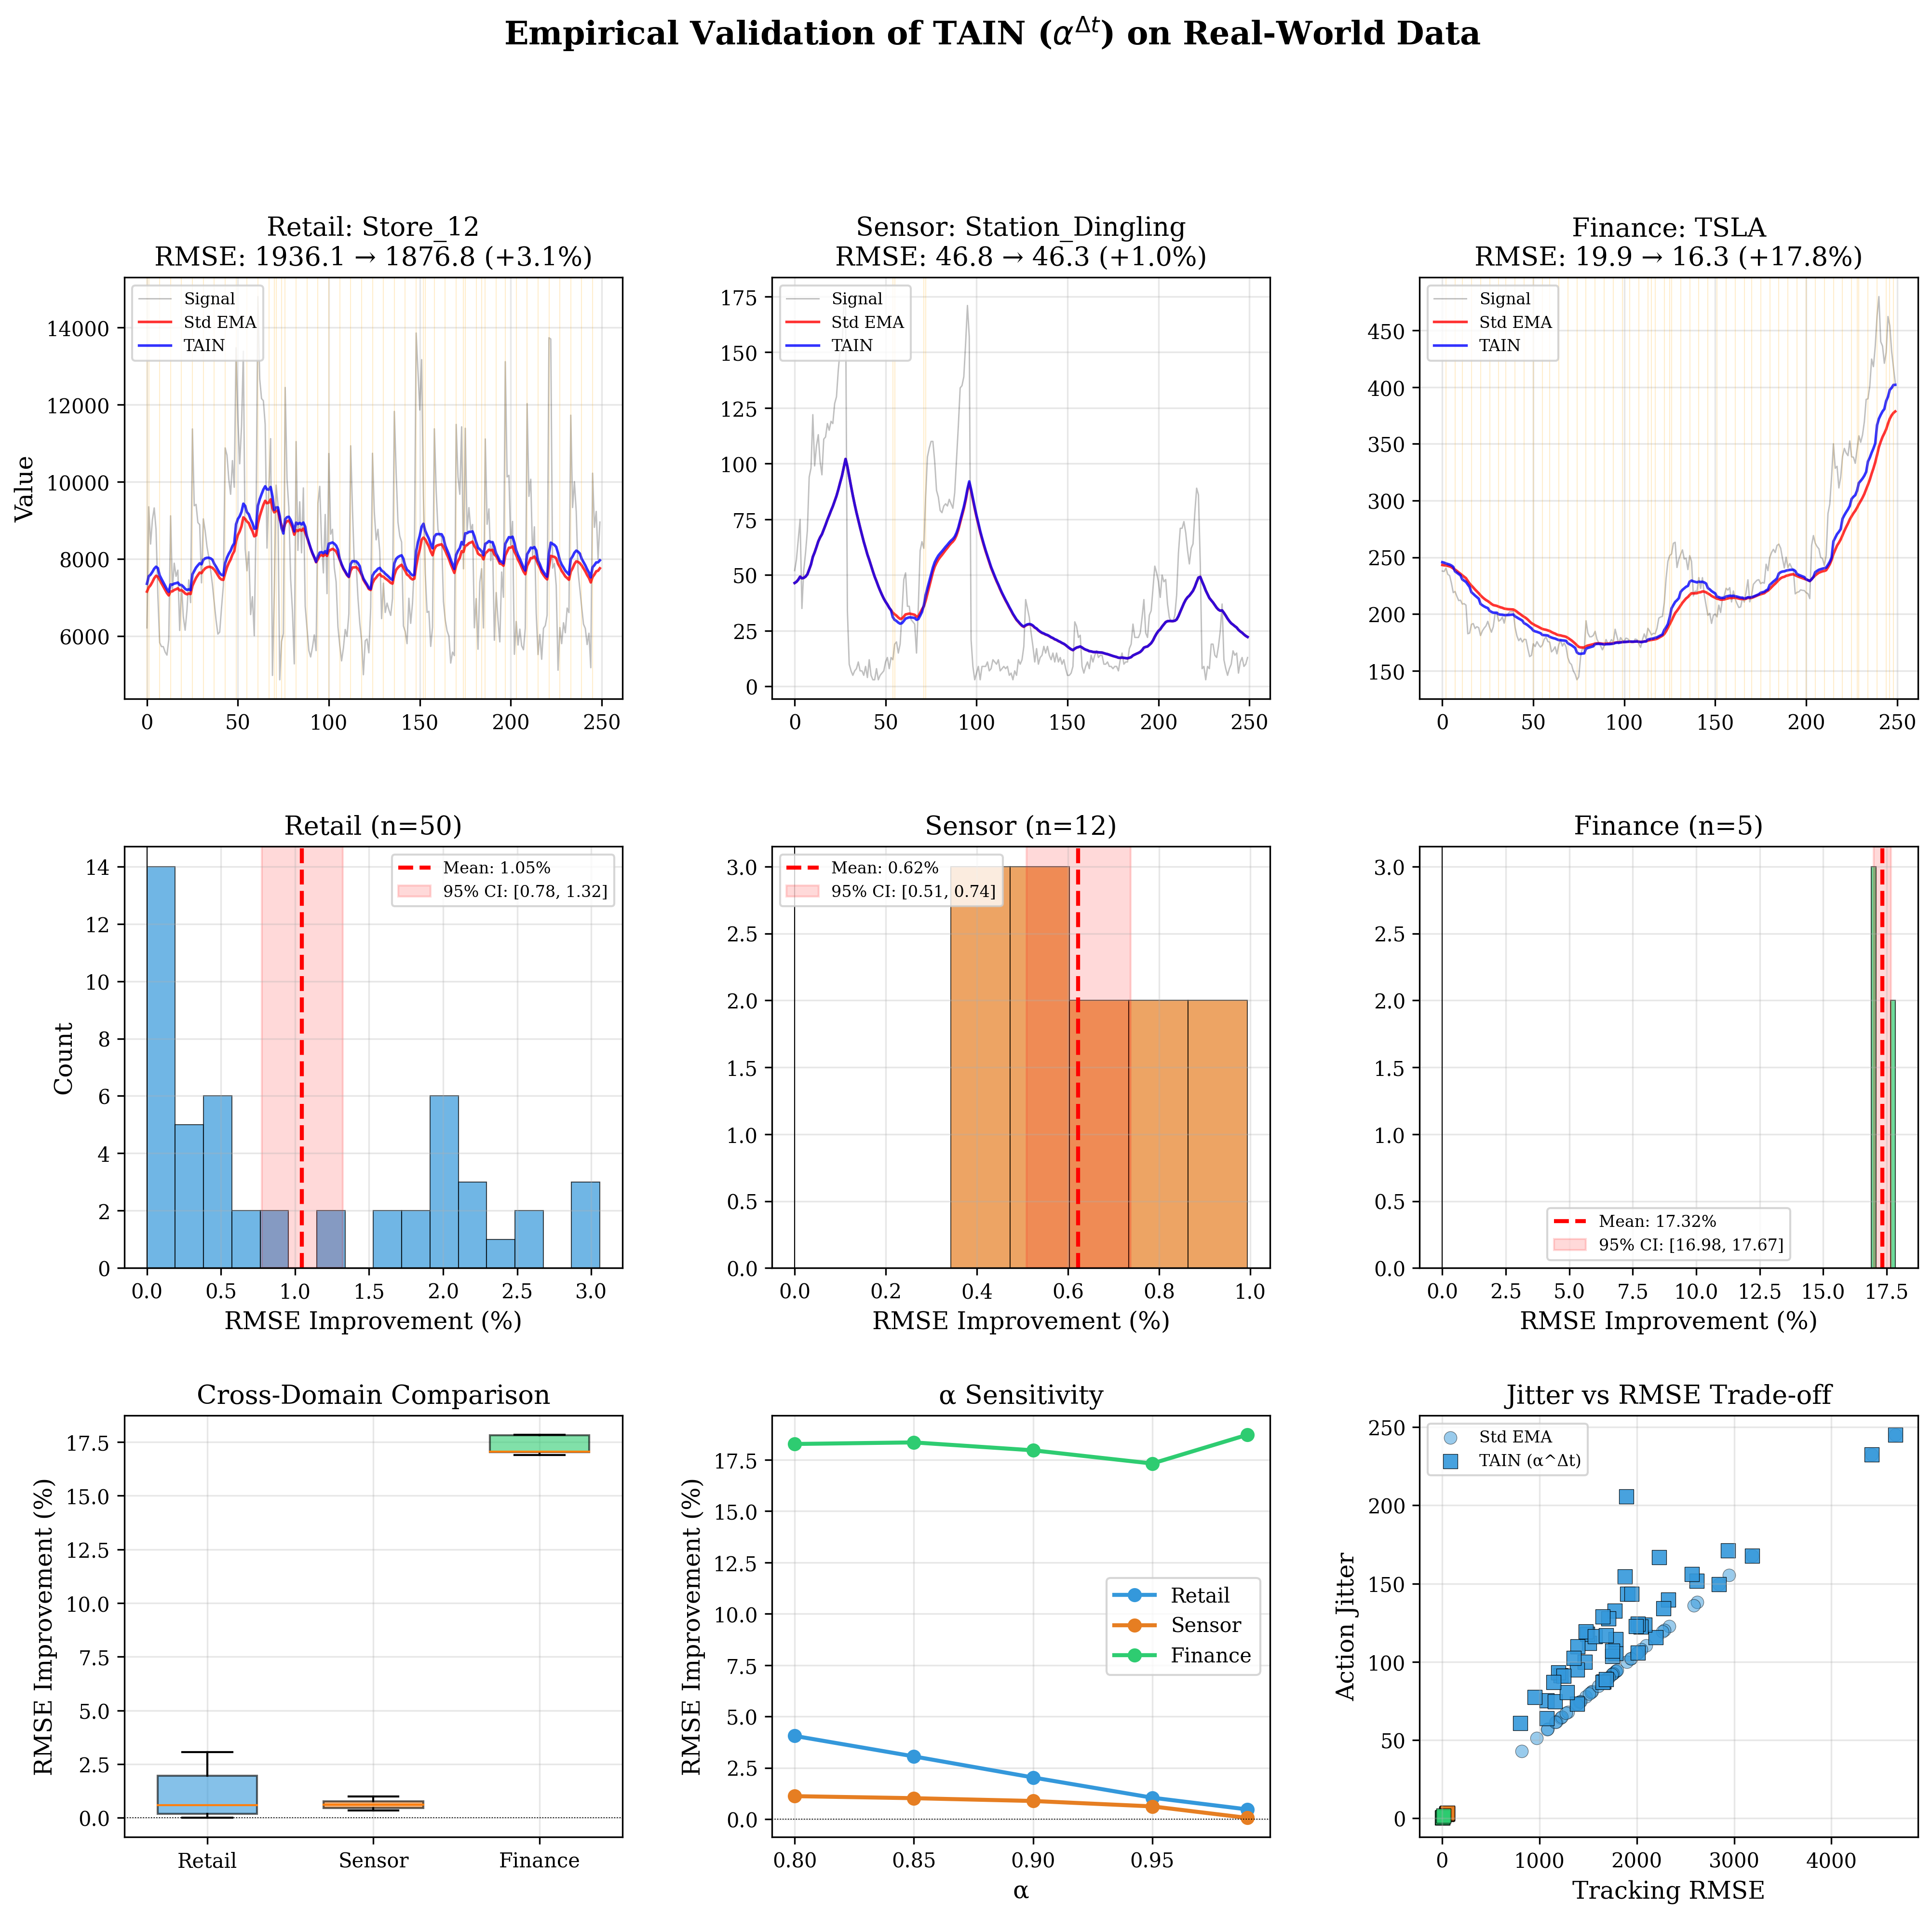
\includegraphics[width=\textwidth]{fig_main_result.png}
\caption{Comprehensive 7-method comparison across five domains. Top row:
tracking examples with gap annotations. Middle row: RMSE distributions.
Bottom row: box plots of J/R ratio, $\alpha$ sensitivity, and RMSE vs.\
Jitter trade-off.}
\label{fig:main_result}
\end{figure}

\begin{figure}[h]
\centering
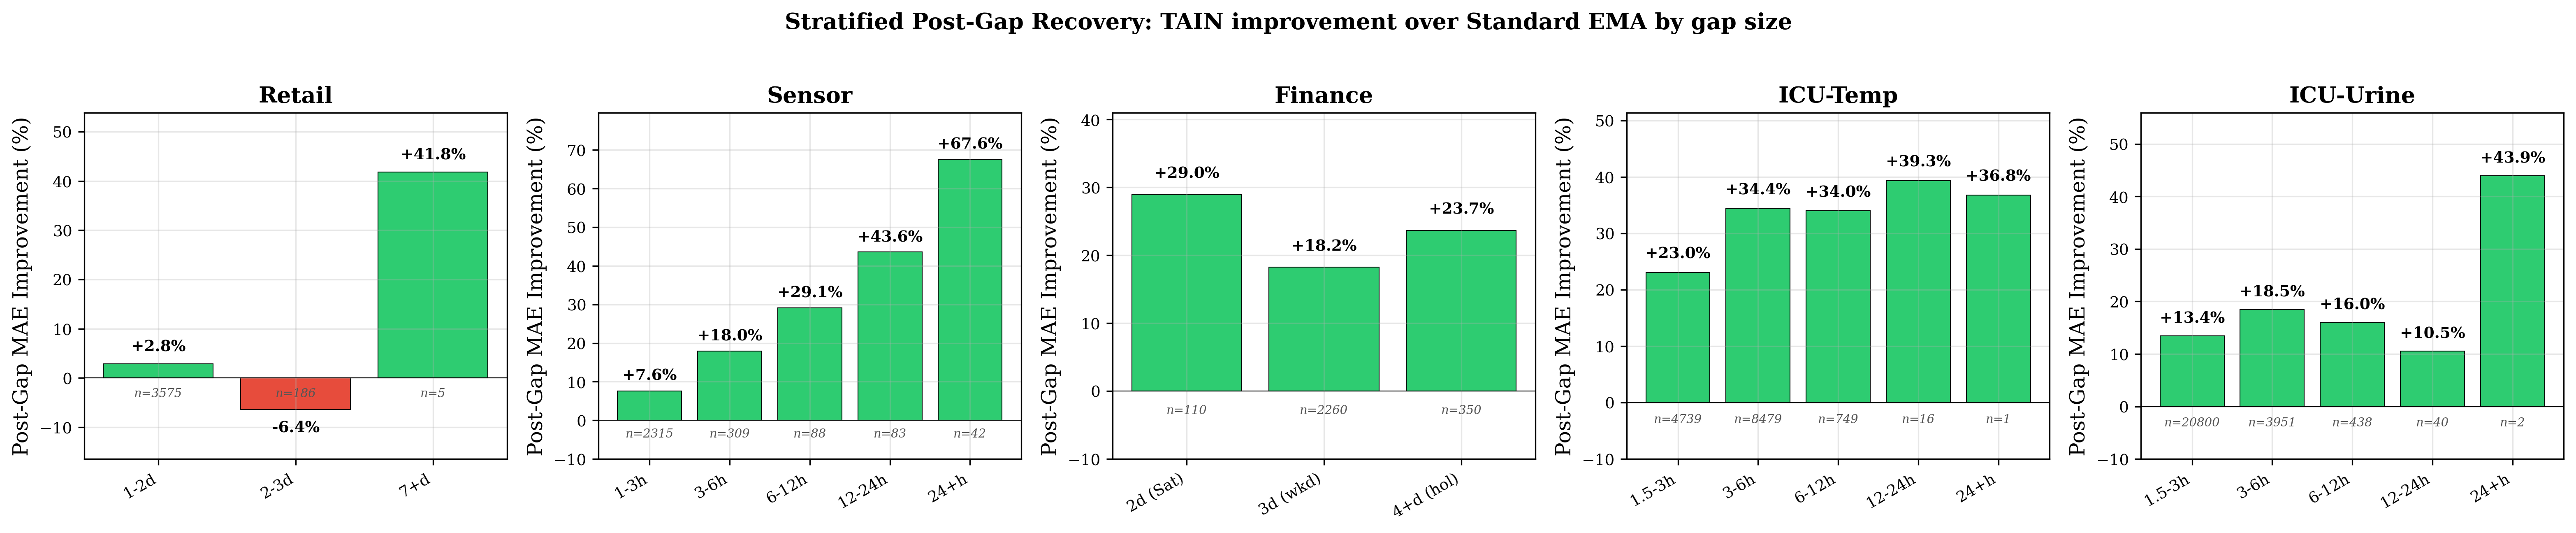
\includegraphics[width=0.85\textwidth]{fig_stratified_gap_recovery.png}
\caption{Stratified post-gap recovery: TAIN improvement (\%) over Standard
EMA as a function of gap size. The sensor domain exhibits a near-perfect
monotonic relationship (7.6\% $\to$ 67.6\%), directly confirming the OU
discretization prediction.}
\label{fig:stratified}
\end{figure}

\begin{figure}[h]
\centering
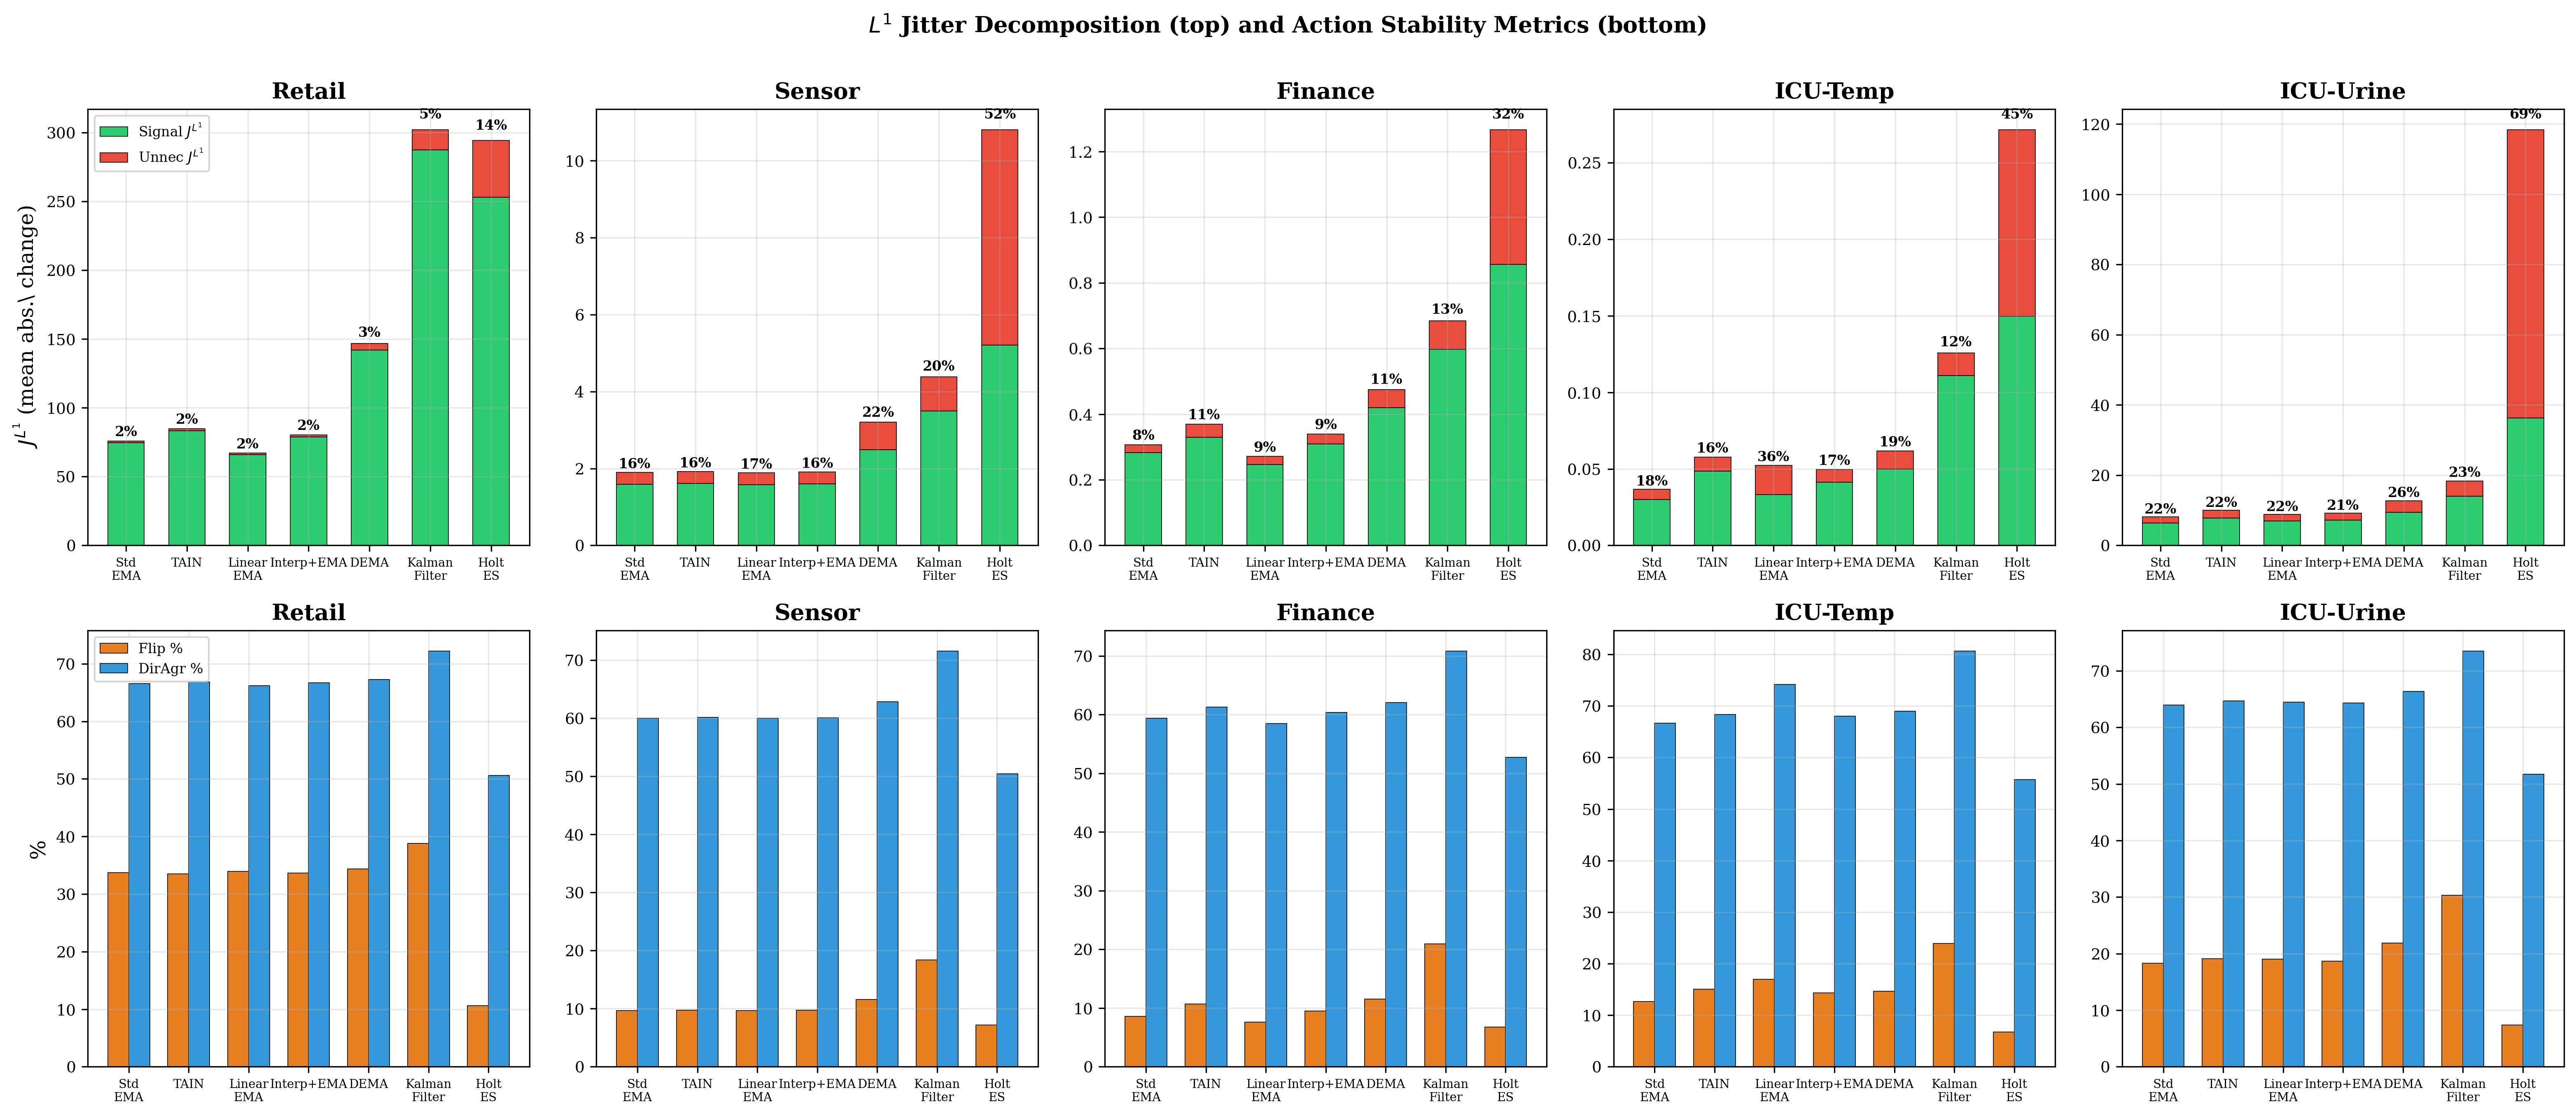
\includegraphics[width=0.85\textwidth]{fig_jitter_decomposition.png}
\caption{$L^1$ jitter decomposition. Left: stacked bar chart showing signal
jitter (desirable) vs.\ unnecessary jitter (undesirable) for each method, with
the unnecessary share annotated. Right: flip rate and directional agreement.
Among RMSE-improving methods, TAIN has the smallest unnecessary-share inflation
over Standard EMA.}
\label{fig:jitter}
\end{figure}

\begin{figure}[h]
\centering
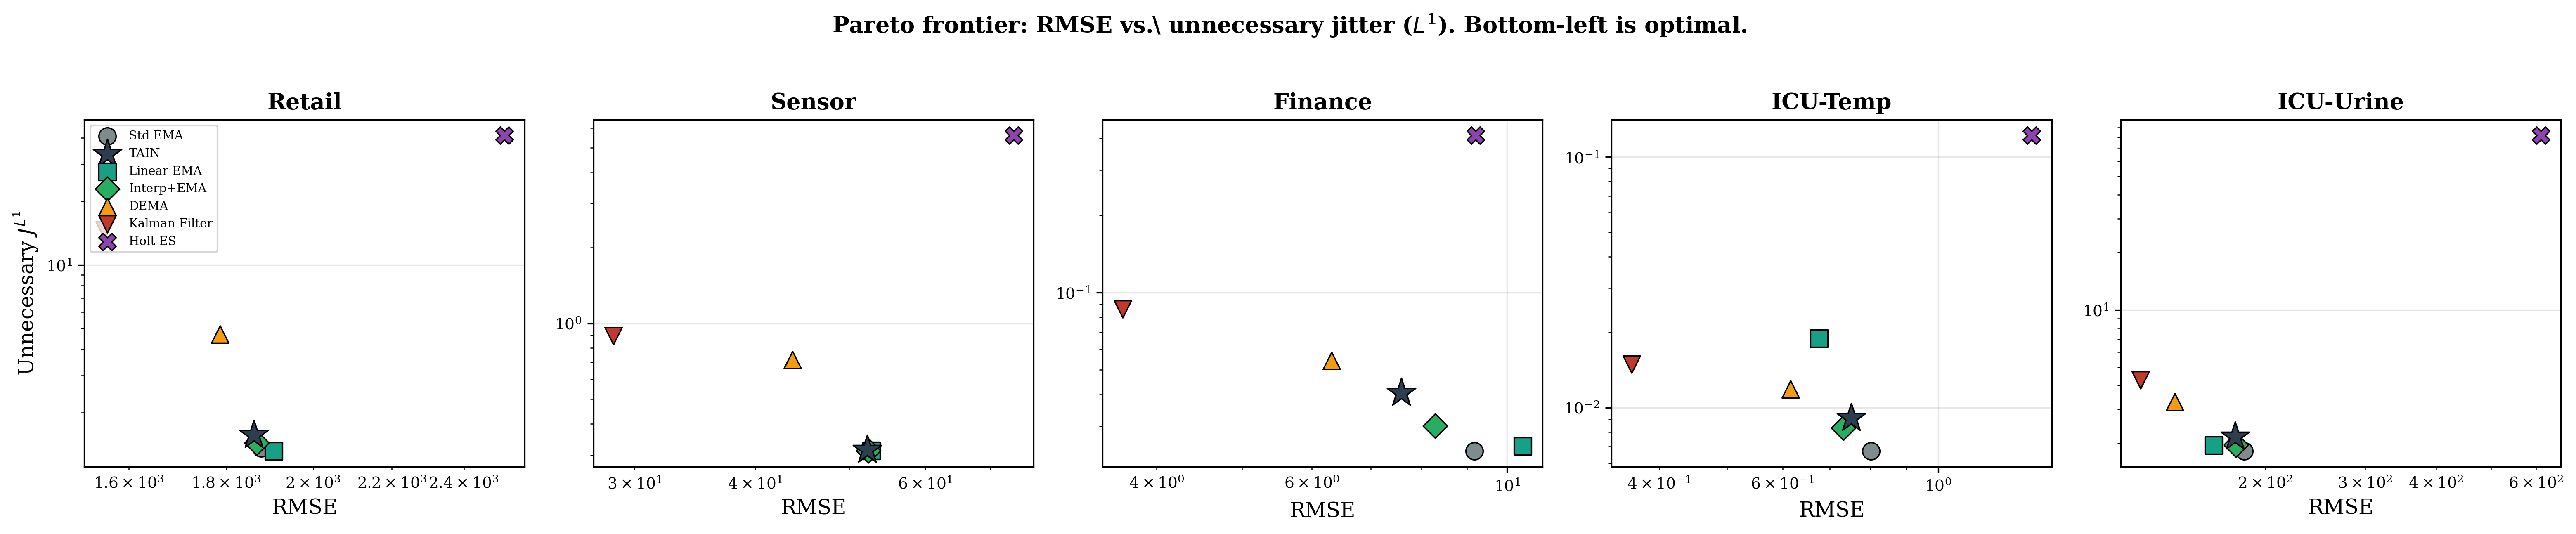
\includegraphics[width=0.85\textwidth]{fig_pareto_rmse_jitter.png}
\caption{Pareto frontier: RMSE vs.\ unnecessary jitter. The bottom-left
corner is optimal. TAIN occupies the Pareto-optimal region in the low-jitter
regime; the Kalman Filter dominates the low-RMSE regime at the cost of
substantially higher action instability.}
\label{fig:pareto}
\end{figure}

\begin{figure}[h]
\centering
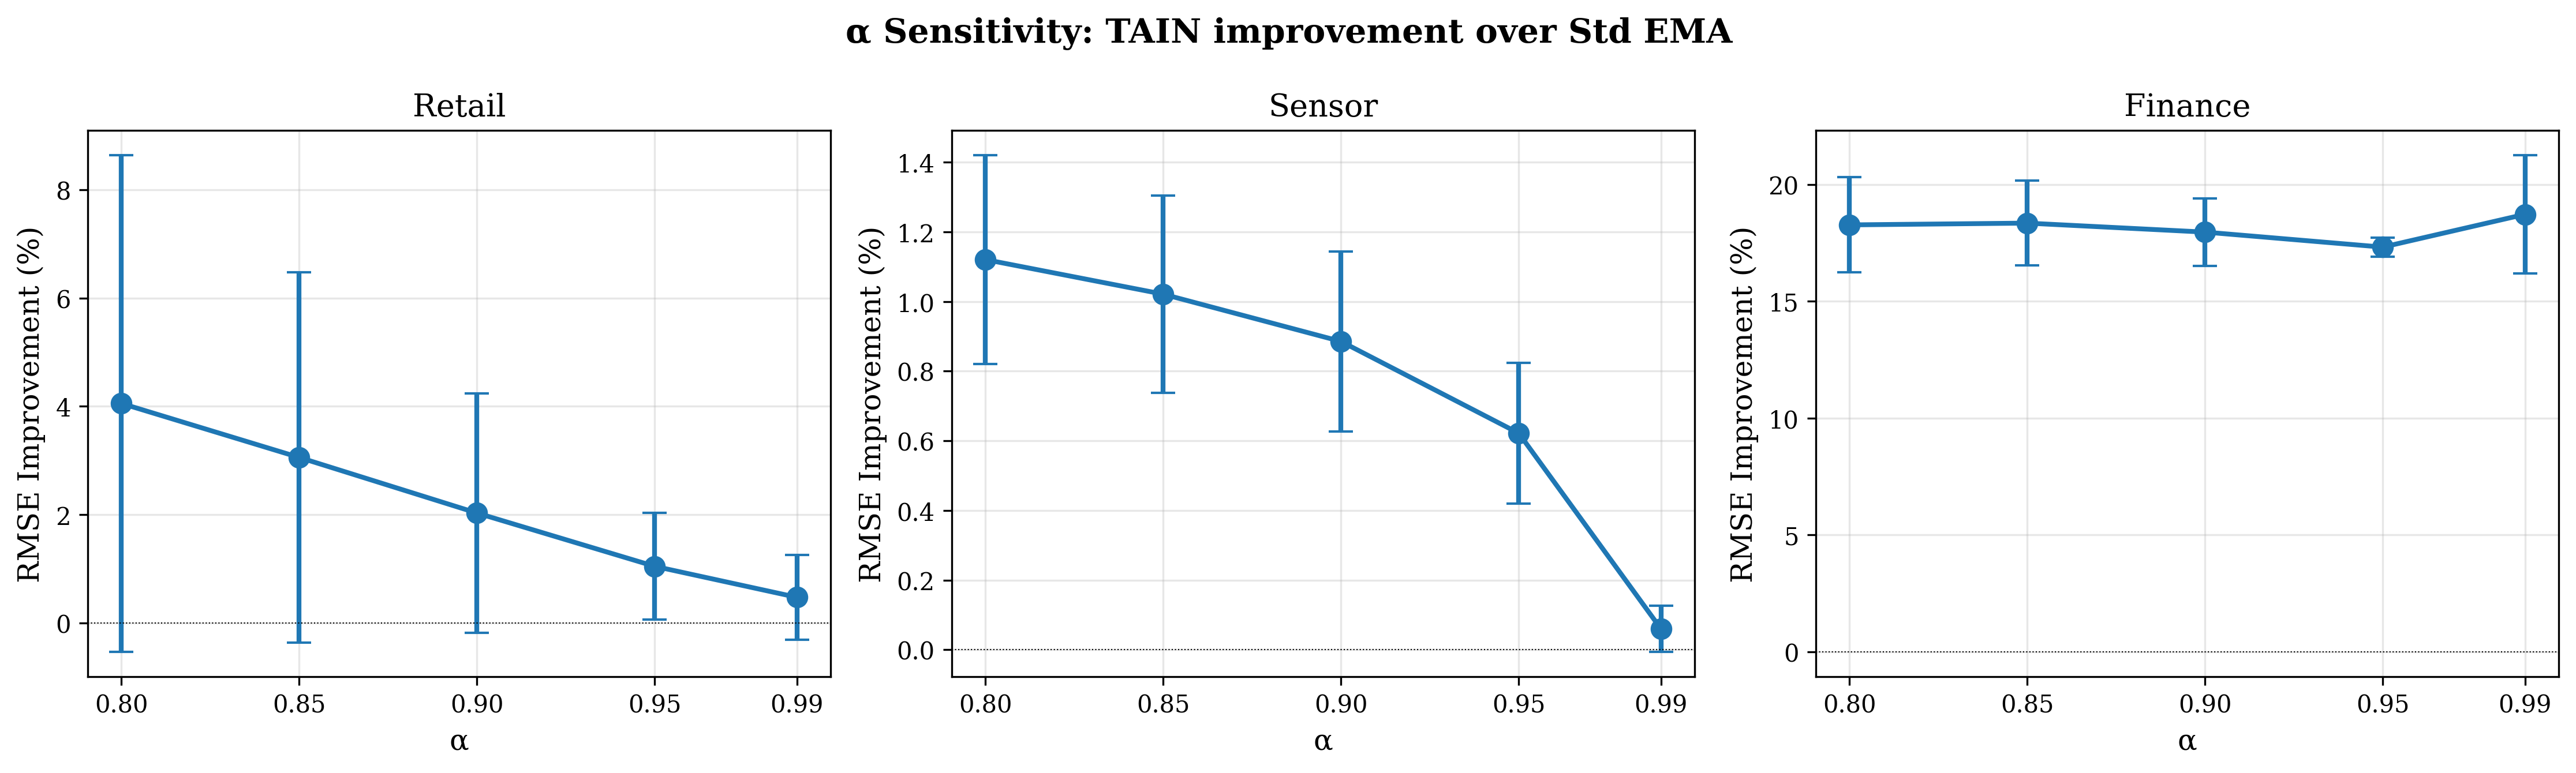
\includegraphics[width=0.85\textwidth]{fig_alpha_sensitivity.png}
\caption{Sensitivity of TAIN's RMSE improvement to the base $\alpha$ parameter.
Improvement is positive across all tested values ($\alpha \in [0.80, 0.99]$)
in all five domains, with lower $\alpha$ producing larger improvements in
Retail and Sensor.}
\label{fig:alpha}
\end{figure}

% ─────────────────────────────────────────────────────────────────────────────
\section{Discussion}

\subsection{Scope of Claims}

This paper makes two types of claims.
\textbf{Mathematical claims} (the OU connection, TAIN convergence, and
gap-proportional recovery) are rigorous and hold under the stated assumptions.
\textbf{Real-world empirical claims} (TAIN's RMSE improvement, post-gap
recovery, and jitter decomposition) are validated on five public datasets
(5{,}409 entities, 659{,}325 observations) with Wilcoxon significance tests and
bootstrap confidence intervals.

The jitter decomposition (Section~5.2.9) reveals that the choice between TAIN and
higher-accuracy methods (e.g., Kalman Filter) is not a question of which is
``better'' but which \emph{operating regime} the deployment requires:
\textbf{high-jitter-tolerant} deployments (automated trading) favor Kalman;
\textbf{low-jitter-required} deployments (retail store management, where action
stability drives operational trust) favor TAIN.

\subsection{Operational Context: Digital Twin Architectures}

In operational digital twin systems, a downstream decision layer (an LLM, a
rule engine, or a human operator) consumes normalized statistics to generate
store-level actions on a daily or weekly cadence. The jitter profile of the
normalization layer directly determines action coherence at this boundary. A
digital twin whose normalization ignores observation gaps propagates
stale-momentum artifacts into the decision layer; the resulting actions oscillate
and erode operator trust. TAIN's gap-proportional reset provides the statistical
hygiene that downstream decision layers require: after a 3-day holiday closure,
running statistics are pulled toward current conditions rather than echoing
pre-closure patterns.

This matters most when the decision layer is an LLM. Language models amplify
input volatility: if the normalized signal oscillates between ``sales rising''
and ``sales falling'' on consecutive days, the LLM generates contradictory
directives (e.g., ``launch a promotion'' followed by ``cancel the promotion'').
By suppressing unnecessary jitter at the normalization stage, TAIN reduces the
risk of such downstream hallucination and keeps the action stream coherent for
the store manager who must act on it.

\subsection{Limitations}

\begin{itemize}[leftmargin=1.5em,itemsep=2pt]
  \item \textbf{Fixed global $\alpha$.} TAIN uses a single $\alpha$ for all
    channels. A per-channel or learned $\alpha_i(t)$ could improve performance,
    particularly for the retail 2--3 day gap reversal.
  \item \textbf{Tracking evaluation only.} TAIN is validated as a running
    statistics tracker, not yet integrated into end-to-end neural network
    training. Integration as a drop-in BatchNorm replacement in architectures
    such as TabNet or FT-Transformer is left to future work.
  \item \textbf{Jitter decomposition requires ground truth.} The unnecessary
    jitter metric requires the true signal $x_t$, limiting its use to evaluation
    settings. An online proxy (e.g., based on rolling statistics) would be needed
    for real-time monitoring.
  \item \textbf{Retail 2--3 day gap reversal.} TAIN shows a $-6.4$\% reversal
    at the 2--3 day gap stratum in the Rossmann dataset, attributable to weekly
    seasonality. Domain-specific or learned $\alpha(t)$ would address this.
  \item \textbf{Strict monotonicity holds only in the Sensor domain.}
    The OU prediction that improvement grows with $\Delta t$ is satisfied at
    the aggregate (largest stratum is best in four of five domains) but with
    within-domain non-monotonicities at intermediate strata (Section~\ref{sec:stratified}).
    Finance offers little gap-size variability (the weekend gap dominates),
    and ICU-Urine shows noise in middle strata. The clean monotonic signature
    requires a domain with both substantial gap-size variation and a relatively
    stationary signal between gaps.
  \item \textbf{Entity-level heterogeneity in ICU-Temp.} The Spearman correlation
    between per-patient mean gap size and per-patient improvement is
    significantly negative ($\rho = -0.139$, $p < 0.001$). This is consistent
    with a patient-acuity confound (sicker patients are sampled more often
    and benefit more from TAIN's fast post-gap correction) rather than a
    failure of the OU discretization, but it indicates that TAIN's gains are
    not uniformly distributed across the cohort. A patient-stratified
    deployment would need to characterize who benefits before generalizing.
\end{itemize}

\subsection{Future Work}

\begin{itemize}[leftmargin=1.5em,itemsep=2pt]
  \item \textbf{End-to-end integration}: replace standard BatchNorm with TAIN
    in production neural network architectures (TabNet, FT-Transformer, NODE)
    and measure downstream task performance.
  \item \textbf{Learned $\alpha(t)$}: address the retail 2--3 day gap reversal
    by learning a context-dependent base decay rate rather than using a fixed
    $\alpha$.
  \item \textbf{Per-channel damping}: extend TAIN to per-channel time-aware
    normalization with a diagonal damping matrix, enabling channel-specific
    viscosity (a direction we term HyperNetwork Viscosity).
  \item \textbf{Stability-gated actions}: combine time-aware normalization with
    a Lyapunov-motivated output gate that suppresses actions during detected
    instability (a direction we term Lyapunov-Gated Action).
  \item \textbf{Online jitter decomposition}: develop a proxy for unnecessary
    jitter that does not require ground truth, enabling real-time action
    stability monitoring.
\end{itemize}

% ─────────────────────────────────────────────────────────────────────────────
\section{Conclusion}

We have introduced \textbf{Time-Aware Inertial Normalization (TAIN)}, a
normalization layer that replaces the fixed EMA coefficient $\alpha$ with
$\alpha^{\Delta t}$, adapting the running statistics' forgetting rate to the
actual elapsed time between observations. While the formula $\alpha^{\Delta t}$
is well established in time series analysis \citep{wright1986,zumbach2001operators},
its application to the normalization layer of neural networks is, to our knowledge,
novel. We ground TAIN in the Ornstein-Uhlenbeck process, providing a principled
theoretical foundation.

To evaluate TAIN's impact on action stability, we employed a \textbf{jitter
decomposition analysis} that separates total action jitter into signal-tracking
(desirable) and unnecessary (undesirable) components, complemented by flip rate
and directional agreement metrics drawn from signal processing and econometrics.
This analytical lens reveals the RMSE--jitter trade-off that existing metrics
(RMSE alone, or total jitter alone) cannot capture.

Empirical validation across five real-world domains (5{,}409 entities, 659{,}325
observations) demonstrates that TAIN achieves statistically significant
improvements over standard EMA ($p < 0.001$ in four of five domains). The
largest gap stratum yields the largest improvement in four of five domains,
with the Sensor domain exhibiting a clean monotonic increase from $+7.6\%$ to
$+67.6\%$ that is a direct empirical signature of the Ornstein-Uhlenbeck
discretization. The $L^1$ jitter decomposition reveals that TAIN's increase
in total jitter over Standard EMA is overwhelmingly signal-tracking rather than
noise (98\%/2\% signal/unnecessary in Retail, $\geq 80\%$ signal across all
five domains).

The empirical case for TAIN rests on three pillars:
\begin{enumerate}
\item \textbf{Statistical significance:} $p < 0.001$ in four of five domains
with 3{,}684/5{,}409 entities (68\%) showing per-entity improvement.
\item \textbf{Gap-proportional recovery:} the largest gap stratum yields the
largest improvement in four of five domains; the Sensor domain shows a clean
monotonic $+7.6\% \to +67.6\%$ progression directly confirming the OU
discretization. Within-domain non-monotonicities at intermediate strata
(Retail 2--3 day reversal, Finance weekend dominance, ICU-Urine middle-stratum
noise) and entity-level heterogeneity (ICU-Temp $\rho = -0.139$, attributable
to patient acuity confound) expose the limits of a single global $\alpha$.
\item \textbf{Efficient signal tracking:} the $L^1$ decomposition shows that
$\geq 80\%$ of TAIN's total-jitter increment over Standard EMA is signal-tracking
across all five domains (98\% in Retail). TAIN's unnecessary-share inflation
over EMA is the smallest among RMSE-improving methods; Kalman and DEMA raise
the unnecessary share by 3--6 pp in every domain and double the flip rate.
\end{enumerate}

More broadly, TAIN serves as the normalization substrate for operational digital
twins. In such architectures, a decision layer (whether an LLM, a rule engine,
or a human operator) consumes the normalized signal to produce daily actions. If
the normalization layer carries stale momentum after an observation gap, the
digital twin loses fidelity to the physical store it mirrors, and every
downstream action inherits that staleness. By resetting running statistics in
proportion to elapsed time, TAIN keeps the digital twin synchronized with
reality across irregular observation schedules.

In retail operations, every unnecessary action change carries a real cost:
cancelled purchase orders, shelf reorganization labor, staff redeployment
friction. These costs are not captured by RMSE or log-likelihood. TAIN-based
normalization minimizes \emph{Operational Churn Cost} (the aggregate cost of
action oscillation), not prediction error alone.

% ─────────────────────────────────────────────────────────────────────────────
\section*{Acknowledgments}

The authors thank the partner retailers for collaboration in defining the
operational requirements that motivated this work. Infrastructure support from
\.{I}T\"{U} \c{C}ekirdek Accelerator, Istanbul, is gratefully acknowledged.

% ─────────────────────────────────────────────────────────────────────────────
\bibliographystyle{plainnat}
\begin{thebibliography}{99}

\bibitem[Chen et al.(2018)]{chen2018neural}
Chen, R.~T.~Q., Rubanova, Y., Bettencourt, J., \& Duvenaud, D. (2018).
\newblock Neural ordinary differential equations.
\newblock \emph{Advances in Neural Information Processing Systems}, 31.

\bibitem[Chen et al.(2021)]{chen2021action}
Chen, C., Tang, H., Hao, J., Liu, W., \& Meng, Z. (2021).
\newblock Addressing action oscillations through learning policy inertia.
\newblock \emph{Proceedings of the AAAI Conference on Artificial Intelligence}.

\bibitem[Che et al.(2018)]{che2018recurrent}
Che, Z., Purushotham, S., Cho, K., Sontag, D., \& Liu, Y. (2018).
\newblock Recurrent neural networks for multivariate time series with missing values.
\newblock \emph{Scientific Reports}, 8(1), 6085.

\bibitem[Choi et al.(2024)]{choi2024tabn}
Choi, J., Lin, J., Chen, Y., Qiu, Q., \& Yu, B. (2024).
\newblock Improving Neural ODE training with temporal adaptive batch normalization.
\newblock \emph{Advances in Neural Information Processing Systems}, 37.

\bibitem[Cipra(2006)]{cipra2006}
Cipra, T. (2006).
\newblock Exponential smoothing for irregular data.
\newblock \emph{Applications of Mathematics}, 51(6), 597--604.

\bibitem[Hasani et al.(2021)]{hasani2021liquid}
Hasani, R., Lechner, M., Amini, A., Rus, D., \& Grosu, R. (2021).
\newblock Liquid time-constant networks.
\newblock \emph{Proceedings of the AAAI Conference on Artificial Intelligence},
  35(9), 7657--7666.

\bibitem[Ioffe \& Szegedy(2015)]{ioffe2015batch}
Ioffe, S., \& Szegedy, C. (2015).
\newblock Batch normalization: Accelerating deep network training by reducing
  internal covariate shift.
\newblock \emph{International Conference on Machine Learning (ICML)}.

\bibitem[Kidger et al.(2020)]{kidger2020neural}
Kidger, P., Morrill, J., Foster, J., \& Lyons, T. (2020).
\newblock Neural controlled differential equations for irregular time series.
\newblock \emph{Advances in Neural Information Processing Systems}, 33.

\bibitem[Mysore et al.(2021)]{mysore2021caps}
Mysore, S., Mabsout, B., Mancuso, R., \& Saenko, K. (2021).
\newblock Regularizing action policies for smooth control with reinforcement learning.
\newblock \emph{IEEE International Conference on Robotics and Automation (ICRA)}.

\bibitem[Silva et al.(2012)]{physionet2012}
Silva, I., Moody, G., Scott, D.~J., Celi, L.~A., \& Mark, R.~G. (2012).
\newblock Predicting in-hospital mortality of ICU patients: The PhysioNet/Computing in Cardiology Challenge 2012.
\newblock \emph{Computing in Cardiology}, 39, 245--248.

\bibitem[Rubanova et al.(2019)]{rubanova2019latent}
Rubanova, Y., Chen, R.~T.~Q., \& Duvenaud, D. (2019).
\newblock Latent ordinary differential equations for irregularly-sampled time
  series.
\newblock \emph{Advances in Neural Information Processing Systems}, 32.

\bibitem[Schaul et al.(2022)]{schaul2022policy}
Schaul, T., Borsa, D., Modayil, J., \& Pascanu, R. (2022).
\newblock The phenomenon of policy churn.
\newblock \emph{Advances in Neural Information Processing Systems}, 35.

\bibitem[Shukla \& Marlin(2021)]{shukla2021multi}
Shukla, S.~N., \& Marlin, B. (2021).
\newblock Multi-time attention networks for irregularly sampled time series.
\newblock \emph{International Conference on Learning Representations (ICLR)}.

\bibitem[Uhlenbeck \& Ornstein(1930)]{uhlenbeck1930theory}
Uhlenbeck, G.~E., \& Ornstein, L.~S. (1930).
\newblock On the theory of Brownian motion.
\newblock \emph{Physical Review}, 36(5), 823--841.

\bibitem[Wright(1986)]{wright1986}
Wright, D.~J. (1986).
\newblock Forecasting data published at irregular time intervals using an
  extension of Holt's method.
\newblock \emph{Management Science}, 32(4), 499--510.

\bibitem[Zumbach \& M\"uller(2001)]{zumbach2001operators}
Zumbach, G., \& M\"uller, U. (2001).
\newblock Operators on inhomogeneous time series.
\newblock \emph{International Journal of Theoretical and Applied Finance},
  4(1), 147--177.

\end{thebibliography}

\end{document}
